\documentclass{iiufrgs}
\usepackage[utf8]{inputenc}
\usepackage{graphicx}
\usepackage[section]{placeins}
\usepackage{setspace}
\usepackage{fontenc}
\usepackage{listings}
\usepackage{color}
\usepackage{url}
\usepackage[printonlyused]{acronym}
\usepackage{rotating}
\usepackage{bytefield}
\usepackage[table]{xcolor}
\usepackage{multirow}
\usepackage{subfigure}
\usepackage{lscape}
\usepackage{enumitem}
\usepackage{fixltx2e}
\usepackage{longtable}
\usepackage{mathtools}
\usepackage{tabularx}
\usepackage{adjustbox}
\usepackage{amsmath}
\usepackage{booktabs}
\usepackage{textcomp}
\usepackage{array}
\usepackage{booktabs}
\usepackage{xcolor}
\usepackage{colortbl}
%\usepackage[brazilian]{babel}
\DeclarePairedDelimiter{\abs}{\lvert}{\rvert}
\onehalfspacing
\urlstyle{sf}
\setdescription{topsep=1em,parsep=0pt,partopsep=0pt,itemsep=0pt}
\setitemize{topsep=1em,parsep=0pt,partopsep=0pt,itemsep=0pt}
\setenumerate{topsep=1em,parsep=0pt,partopsep=0pt,itemsep=0pt}
\lstset{frame=tb,
  language=Java,
  aboveskip=3mm,
  belowskip=3mm,
  showstringspaces=false,
  columns=flexible,
  basicstyle={\small\ttfamily},
  numbers=none,
  numberstyle=\tiny\color{gray},
  keywordstyle=\color{blue},
  commentstyle=\color{dkgreen},
  stringstyle=\color{red},
  breaklines=true,
  breakatwhitespace=true,
  tabsize=3
}

\course{\cgcc}
\title{O Uso de Processamento de Linguagem Natural para a Análise de
Sentimentos na Rede Social Reddit.}
\author{Santos Andreata}{Guilherme Henrique}
\advisor[]{Martinotto}{André Luis}
\location{Caxias do Sul}{}
\bibpunct{(}{)}{;}{a}{,}{,}

\begin{document}

\maketitle  

\begin{titlepage}
%\setcounter{page}{2} - Inclui o número da página
%\thispagestyle{headings}
\vfill

\begin{center}
{\setlength{\unitlength}{1cm}\makebox(12,6.5){\parbox[c]{12cm}{\setlength{\parskip}{0.8cm}\center\vskip -1.2cm\LARGE{\bf O Uso de Processamento de Linguagem Natural para a Análise de Sentimentos na
Rede Social Reddit.}\par \normalsize por\par \large Guilherme Henrique
Santos Andreata\par}}}
\end{center}

{\large Projeto de Diplomação submetido ao curso de Bacharelado em Sistemas de
Informação da área de conhecimento de ciências exatas e engenharia, como requisito obrigatório para graduação.}

\vfill

\begin{center}
{\Large\bf Projeto de Diplomação}
\end{center}

\vfill

\begin{singlespace}
Orientador: {André Luis Martinotto\par}

Banca examinadora:\par
\hspace{1cm} {\setlength{\unitlength}{1cm}
\makebox(9,1){\parbox[c]{9cm}{\center Daniel Luis Notari\\ CCTI/UCS}}}\par
\hspace{1cm} {\setlength{\unitlength}{1cm}
\makebox(9,1){\parbox[c]{9cm}{\center Helena Graziottin Ribeiro\\ CCTI/UCS}}}\par

\vfill

%\hfill{\setlength{\unitlength}{1cm}\makebox(9,2.5){\parbox[c]{9cm}{\setlength{\parskip}{0.8cm}\center\vskip
% -1.2cm Projeto de Diplomação apresentado em\\ 5 de Dezembro de 2013\par Daniel Luís Notari\\ Coordenador}}}

\end{singlespace}

\end{titlepage}

\tableofcontents

\chapter*{Lista de acrônimos}

\vspace{20px}
\begin{acronym}[XXXXXXXXXX]
\acro{NLP}[NLP]{\textit{Natural Language Processing}}
\acro{NLTK}[NLTK]{\textit{Natural Language Toolkit}}
\acro{MaxEnt}[MaxEnt]{\textit{Maximum Entropy}}
\acro{RNTN}[RNTN]{\textit{Recursive Neural Tensor Networks}}
\acro{VADER}[VADER]{\textit{Valence Aware Dictionary and sEntiment Reasoner}}
\acro{JSON}[JSON]{\textit{JavaScript Object Notation}}
\acro{POJO}[POJO]{\textit{Plain Old Java Objects}}
\acro{SVM}[SVM]{\textit{Support Vector Machines}}
\end{acronym}
\listoffigures
\listoftables

\keyword{Reddit}
\keyword{Processamento de Linguagem Natural}
\keyword{Análise de Sentimentos}

\begin{abstract}

Nos tempos atuais, a sociedade tem cada vez mais se expressado através de Redes
Sociais, dentre várias redes sociais, se destaca o Reddit, no qual além de ser
uma das maiores redes sociais no mundo, é uma rede social de \textit{links},
aonde usuários postam e comentam sobre estes gerando um grande volume de dados que muitas vezes se dão por
ignorados.

A identificação de padrões de sentimentos expressos por grupos dessa comunidade, se faz útil visto que a partir dessa avaliação é possível construir ferramentas que apoiam decisões tanto de um ponto de vista político, como por
exemplo, entender qual é a opinião sobre um determinado assunto de um conjunto
de eleitores, tanto quanto um ponto de vista de negócios, para entender qual a
opinião dos consumidores de um produto, ou de seu competidor, a respeito de um
determinado assunto.

Neste volume serão apresentados estudos sobre o Processamento de Linguagem
Natural e Análise de Sentimentos, os quais apresenta o objetivo da criação de um
\textit{software} no qual seja possível efetuar a análise de sentimentos na rede
social Reddit.

\end{abstract}


\acresetall

\chapter{Introdução}
\label{chap:introducao}
A linguagem é a forma com que nós nos comunicamos, seja ela escrita ou
falada, através de símbolos ou sons. De fato, a linguagem é a forma como
expressamos nossas idéias, sentimentos e experiências. O Processamento de
Linguagem Natural, é o termo utilizado para descrever um software ou componente
de hardware que tem como função analisar a linguagem escrita ou falada
\cite{jacksonmoulinier2007}.

Existem duas abordagens de Processamento de Linguagem Natural, sendo a primeira
delas é chamada de simbólica ou racionalista e a outra de empírica. A primeira
abordagem consiste em uma série de regras para a manipulação de símbolos, como as regras gramaticais que permitem identificar se uma frase está malformada ou não. A abordagem
empírica está centrada na análise estatística da linguagem através de grandes quantidades
de textos, como por exemplo, a utilização de modelos de Markov para reconhecer padrões
na escrita \cite{jacksonmoulinier2007}.

Existem diversos \textit{frameworks open source} que facilitam o desenvolvimento
de \textit{software} para o Processamento de Linguagem Natural, sendo que entre
esses destacam-se o \textit{Stanford's Core NLP Suite} \cite{corenlp}, \textit{Natural Language
Toolkit} \cite{nltk}, \textit{Apache OpenNLP} \cite{opennlp} e \textit{Spacy}
\cite{spacy}.
Esses \textit{frameworks} nos permitem, entre outras coisas, efetuar análise de
sentimentos, identificar tópicos e conteúdos.

A rede social Reddit é o vigésimo terceiro \textit{website} mais acessado na
internet e o sétimo mais acessado nos Estados Unidos da América \cite{alexa}.
Através deste \textit{website}, seus usuários podem criar ou se inscrever em
comunidades, também conhecidas como \textit{subreddits}.
Uma vez que as comunidades são criadas pelos próprios usuários, podemos encontrar
comunidades sobre todos os assuntos, sejam notícias do mundo, comunidades
partidárias, comunidades criadas para pessoas de uma mesma localidade ou comunidades
de imagens engraçadas.

Nestas comunidades é possível visualizar e comentar \textit{links} enviados por
outros usuários.
Além disso, o usuário pode efetuar um voto de forma positiva, caso acredite que
aquele \textit{link} é útil para a comunidade. Caso contrário, é possível
efetuar um voto negativo.
Uma vez que os próprios usuários podem submeter \textit{links}, os eventos e
notícias de todo o mundo são reportados no \textit{website}, como exemplo,
pode-se citar as eleições ocorridas no ano de 2016 nos Estados Unidos e o
tiroteio ocorrido em Paris.

Neste trabalho será desenvolvido um software que permita realizar a
análise dos comentários do \textit{website} Reddit. Mais
especificamente esses comentários serão analisados com o objetivo de identificar padrões de sentimentos, ou seja, determinar se a
opinião expressada com relação a um determinado tópico é neutra, positiva ou negativa.

\section{Objetivos do Trabalho}

Este trabalho tem como objetivo a análise dos comentários disponíveis no
\textit{website} Reddit, identificando padrões de sentimentos entre os
usuários de suas comunidades. De forma a atingir o objetivo principal desse
trabalho, os seguintes objetivos específicos devem ser realizados:
\begin{itemize}
  \item Desenvolver uma ferramenta para o Processamento Natural de Linguagem através de
\textit{frameworks} já existentes.
 \item Construção de uma base de dados a partir do \textit{website} Reddit.
 \item Efetuar o processamento da base de dados utilizando a ferramenta desenvolvida.
\end{itemize}

\section{Estrutura do Trabalho}
%O presente trabalho está estruturado da seguinte forma: no Capítulo
% \ref{cap:Animacao} será apresentada a história da animação, seu surgimento e conceitos. No Capítulo \ref{cap:Blender} são apresentadas informações sobre o \textit{software} Blender, assim como os métodos disponíveis nesse para a criação de animações 3D. No Capítulo \ref{cap:Kinect} será apresentado o sensor Kinect, assim como seu funcionamento e alguns conceitos sobre as imagens capturadas. No Capítulo \ref{cap:DesenvKinect} serão apresentadas as bibliotecas e ferramentas para o desenvolvimento de aplicações utilizando Kinect. Além disso, é realizado um comparativo, onde são apresentadas as vantagens e desvantagens de cada uma dessas ferramentas. No Capítulo \ref{cap:AplicaIntegra} serão apresentados alguns \textit{softwares} que já fazem a integração entre o sensor e a ferramenta, assim como o funcionamento desses. No Capítulo \ref{cap:Implementacao} serão apresentados os detalhes da solução desenvolvida e da animação gerada, bem como são apresentados os testes realizados e os resultados obtidos. Por fim, no Capítulo \ref{cap:Consideracoes} são apresentadas as considerações finais e sugestões de trabalhos futuros.

\chapter{Processamento de Linguagem Natural}
\label{cap:Processamento}

% Um computador, obviamente, está preparado para entender sua própria linguagem,
% como por exemplo, um compilador interpreta linhas de código fonte para gerar um
% programa executável seguindo exatamente o algoritmo utilizado. Por isso, temos o
% termo Natural no Processamento de Linguagem. 

O objetivo da área de Processamento de Linguagem Natural é analisar a linguagem natural, ou seja, a linguagem utilizada pelo seres humanos não
importando se essa é escrita ou falada \cite{manningschutze1999}.

O Processamento de Linguagem Natural é uma área antiga, sendo anterior a
invenção dos computadores modernos. De fato, sua primeira grande aplicação foi
um dicionário desenvolvido no Birkbeck College em Londres no ano de 1948. Por ser
uma área complexa, seus primeiros trabalhos foram notavelmente falhos o que
causou uma certa hostilidade por parte das agências formentadoras de pesquisas.

Os primeiros pesquisadores eram muitas vezes bilíngues, como por exemplo,
nativos alemães que imigraram para os Estados Unidos. Acreditava-se que pelo
fato desses terem conhecimento de ambas as linguas, Ingles e Alemão, eles teriam
capacidade de desenvolver programas de computadores que efetuariam a tradução das linguas
de modo satisfatório. Uma vez que esses encontraram muitas dificuldades,
ficou claro que o maior problema não era o conhecimento de ambas as
línguas e sim como expressar esse conhecimento na forma de um programa de
computador \cite{history}.

Para que um computador seja capaz de interpretar uma
língua, necessitamos antes entender como nós efetuamos essa
interpretação.
Por isso, uma parte considerável do Processamento de Linguagem Natural está apoiado na área de Linguística.

\section{Linguística}

O objetivo da Linguística é compreender como os humanos adquirem, produzem e
entendem as diversas línguas, ou seja, a forma com que conversamos, a nossa
escrita e outras mídias de comunicação \cite{manningschutze1999}.

Na linguagem tanto escrita, como na falada, existem regras que são utilizadas
para estruturar as expressões. Uma série de dificuldades no Processamento de
Linguagem Natural são ocasionadas pelo fato de que as pessoas constantemente
mudam essas regras para satisfazerem suas necessidades de comunicação
\cite{manningschutze1999}. Uma vez que as regras são constantemente modificadas pelo loucutor, se torna extremamente difícil a criação de um software ou hardware efetue a interpretação de uma língua. 


% \subsection{Sintaxe e Semântica}
% 
% No seu livro Estruturas Sintáticas, Noam Chomsky cita as seguintes frases
% ``Ideias verdes incolores dormem furiosamente'' e ``Incolores verde ideias dormem
% furiosamente''.
% 
% A primeira frase, do ponto de vista sintático é correta, porém, assim como a
% segunda frase, semânticamente não faz sentido.
% 
% O fato de que podemos modificar as regras da lingua de duas formas distintas é
% utilizado como evidência para a separação da sintaxe e semântica na língua.
% \cite{jacksonmoulinier2007}

\section{Métodos de Processamento de Linguagem Natural}

O \ac{NLP} tem como o objetivo a execução de diversas tarefas como categorização
de documentos, tradução e geração de textos a partir de um banco de dados de
computador, etc. Podemos destacar duas formas ou métodos para a execução dessas
tarefas, o método simbólico e o método estatístico, com origem o campo da linguística. 

Nos final dos anos 50 e 60, existiam excelentes métodos quantitativos
desenvolvidos durante a segunda guerra mundial para a solução de problemas
científicos \cite{shannon48}.
Porém, no ano de 1957, Chomsky publicou o seu trabalho ``Syntactic Structures''
e com isso, temos a primeira aparição da teoria de gramática gerativa, que
considera a gramática como um conjunto de regras. Essa abordagem através de um
conjunto de regras ao invés de um modelo matemático entra em conflito com os
trabalhos anteriores, criando duas comunidades no campo de Linguística. Como
reflexo das duas comunidades, a área de \ac{NLP} que crescia em paralelo a
linguística também foi dividida em duas, uma área que fazia uso de métodos que
utilizavam regras(simbólico) e uma outra área que fazia uso de métodos
quantitativos(estatísticos).


Essa seção tem como objetivo explicar os dois métodos principais de
abordagem e demonstrar as diferenças entre os dois métodos através de um exemplo
de desambiguação de categoria de palavras.


\subsection{Método Simbólico} 
O método simbólico ou racionalista está
baseado no campo da Linguística e faz o uso da manipulação dos símbolos,
significados e das regras de um texto. Um exemplo de método simbólico é o
método de Brill \cite{Brill:1992:SRP:974499.974526}. Por exemplo, no método de
Brill a frase ``João pintou a casa de branco'', será separada em palavras que
serão classificadas através de um dicionário pré-definido, como:

\begin{table}[htb]
\centering
\begin{tabular}{l|l|l|l|l|l|l}
Palavra         & João        & pintou & a      & casa        & de        
& branco
         \\
%Correta: & Substantivo & Verbo  & Artigo & Substantivo & Preposição &
% Substantivo \\
Classificação:   & 			   & Verbo  & Artigo & Substantivo & Preposição & Adjetivo
\end{tabular}
\label{my-label}
\end{table}

Observa-se que algumas palavras não foram
identificadas, como ``João'' ou classificadas de forma errada, como
``branco". Desta forma, o método utiliza-se de outras duas regras para uma
classificação inicial.
A primeira regra classifica todas as palavras desconhecidas que iniciam em
maiúsculo como substantivos, por exemplo, a palavra ``João''. Já a segunda regra, atribui para a palavra desconhecida a mesma classificação
de outras palavras que terminam com as mesmas três letras. Por exemplo, supondo
que a palavra ``pintou'' não fosse encontrada no dicionário, essa seria
associada a outras palavras terminadas com o sufixo ``tou''. Ou seja, essa seria
associada como verbo.

\begin{table}[htb]
\centering
\begin{tabular}{l|l|l|l|l|l|l}
Palavra         & João        & pintou & a      & casa        & de        
& branco
         \\
%Correta: & Substantivo & Verbo  & Artigo & Substantivo & Preposição &
% Substantivo \\
Classificação:   & \textbf{Substantivo} & Verbo  & Artigo & Substantivo &
Preposição & Adjetivo
\end{tabular}
\label{my-label}
\end{table}



Após essa classificação inicial, o método executa o seguinte conjunto de regras:

\begin{itemize}
   \item Se uma palavra tem a classificação \textbf{A} e está no contexto
  \textbf{C} então a sua classificação deverá ser mudada para \textbf{B}. Por
  exemplo, se uma palavra \textbf{A} (branco no exemplo) é um adjetivo e uma das
  duas palavras anteriores é uma preposição (``de'' no contexto \textbf{C}
  ), mude para sua classificação para substantivo (classificação \textbf{B}).
  
  \[\overbrace{\text{João}}^\text{Substantivo}
  \overbrace{\text{pintou}}^\text{Verbo}
  \overbrace{\text{a}}^\text{Artigo}
  \underbrace{
  \overbrace{\text{casa}}^\text{Substantivo}
  \overbrace{\text{de}}^\text{Preposição}}_\text{Contexto \textbf{C}}
  \underbrace{\overbrace{\text{branco}}^{\textcolor{red}{Adjetivo}}}_\text{Classificação
  \textbf{A}\textrightarrow\textbf{B}}
 \]
 
  \item Se uma palavra tem a classificação \textbf{A} e tem uma propriedade
  \textbf{P} então a sua classificação deverá ser alterada para \textbf{B}. Por
  exemplo, se uma palavra \textbf{A} (``Linda'') foi classificada como um
  adjetivo e é iniciada com uma letra maiúscula (propriedade \textbf{P}), sua
  classificação deverá ser alterada para substantivo (classificação \textbf{B}).
  
  \[\overbrace{\text{Comprei}}^\text{Verbo}
  \overbrace{\text{flores}}^\text{Substantivo}
  \overbrace{\text{para}}^\text{Preposição}
  \underbrace{\overbrace{\text{L}\text{inda}}^{\textcolor{red}{Adjetivo}}}_\text{Classificação
  \textbf{A}\textrightarrow\textbf{B}}
 \]
 
  \item Se uma palavra tem a classificação \textbf{A} e uma palavra com a
  propriedade \textbf{P} está na região \textbf{R}, sua classificação deverá
  ser \textbf{B}. Por exemplo, se uma das duas palavras anteriores (``João
  adora" na região \textbf{R}) iniciam com letra maiúscula (propriedade
  \textbf{P}), sua classificação deverá ser alterada para substantivo (classificação \textbf{B}).
  
   \[\underbrace{\overbrace{\text{João}}^\text{Substantivo}
  \overbrace{\text{adora}}^\text{Verbo}}_\text{Região \textbf{R}}
  \underbrace{\overbrace{\text{L}\text{inda}}^{\textcolor{red}{Adjetivo}}}_\text{Classificação
  \textbf{A}\textrightarrow\textbf{B}}
 \]
 
  
\end{itemize}

\subsection{Método Estatístico} 
O método estatístico ou empírico utiliza-se de grandes
quantidades de texto, procurando por padrões e
associações a modelos, sendo que esses podem ou não estarem relacionados com
regras sintáticas ou semânticas. Como exemplo, podemos citar a utilização de
Modelos de Markov pela algoritmo de Viterbi. Onde, a partir de um conjunto de
dados já classificados, ou seja, um \textit{training set} é verificada a
possibilidade de transição entre as classes gramaticais.
Por exemplo, se no nosso \textit{training set}, temos 10000 substantivos que em
7000 dos casos são seguidos por um verbo, temos:

\[ P(VB|SM) = \frac{C(SM,VB)}{C(SM)} = \frac{7000}{10000} = 0.7 \]

Onde \textbf{VB} são verbos e \textbf{SM} substantivos. Como pode ser observado
na equação, a probabilidade de um substantivo ser seguido de um verbo
(\textbf{(VB$\vert$SM)}) é igual a ocorrência de substantivos seguidos de verbos (\textbf{C(SM,VB)})
dividida pela quantidade total de substantivos em nosso \textit{training set}.

Após, é calculada a probabilidade de cada palavra ser associada com uma classe.
Supondo que dos 10000 substantivos, 150 são a palavra ``um'' classificada
dentre artigo, substantivo e pronome, como substantivo:

\[ P(um|SM) = \frac{C(SM,um)}{C(SM)} = \frac{150}{10000} = 0.015 \]

Aonde que \textbf{um} é a palavra que está sendo classificada e \textbf{SM}
são os substantivos existentes no nosso \textit{training set}. Portanto a
probabilidade de um substantivo ser associada a palavra ``um''
(\textbf{P(um$\vert$SM)}) é igual a quantidade da palavra ``um''
classificada como substantivo (\textbf{C(SM,um)}) dividida pela quantidade de
substantivos em nosso \textit{training set}.
Como exemplo, vamos supor os seguintes dados compilados através dos dois métodos
citados anteriormente, aonde a primeira tabela representa a probabilidade de
transição e a segunda tabela representa a probabilidade de associação:

\begin{table}[htb]
\centering
\begin{tabular}{|l|l|l|l|l|}
\hline
            & Substantivo & Verbo & Artigo & Pronome \\ \hline
Início      & 0.30        & 0.25  & 0.35   & 0.4     \\ \hline
Substantivo & 0.4         & 0.2   & 0.015  & 0.85    \\ \hline
Verbo       & 0.5         & 0.2   & 0.3    & 0.07    \\ \hline
Artigo      & 0.1         & 0.001 & 0.030  & 0.005   \\ \hline
Pronome     & 0.7         & 0.005 & 0.005  & 0.8     \\ \hline
\end{tabular}
\caption{Tabela de Probabilidade de Transição}
\label{tabela:transicao}
\end{table} 

\begin{table}[htb]
\centering
\begin{tabular}{|l|l|l|l|l|}
\hline
            & João & comprou & um    & carro \\ \hline
Substantivo & 1    &         & 0.015 & 1     \\ \hline
Verbo       &      & 1       &       &       \\ \hline
Artigo      &      &         & 0.030 &       \\ \hline
Pronome     &      &         & 0.005 &       \\ \hline
\end{tabular}
\caption{Tabela de Probabilidades de Associação}
\label{tabela:associacao}
\end{table}


Portanto, para a classificação da frase anterior, as palavras João, Comprou
e Carro, só podem ser classificadas como substantivo (SM), verbo (VB) e
substantivo (SM) respectivamente. Porém, a palavra ``um" pode ser classificada
em substantivo (SM), artigo (ART) e pronome (PRO). A seguinte imagem representa
as possibilidades de caminho que o classificador pode percorrer neste exemplo:

\begin{figure}[htbp]
 \centering
 \includegraphics[height=180px]{imagens/markov.png}
 \caption{Caminhos possíveis de classificação}
 \label{fig:markov}
\end{figure}

\newpage
Para a identificação da classe da palavra ``um'' é realizada a seguinte equação
seguindo o caminho representado pela figura anterior, começando pela palavra
João:

\[ v_t(j) = v_{t-1} a_{ij} b_j(o_t) \]

Aonde que $v_t$ é a probabilidade do caminho atual, $v_{t-1}$ é a
probabilidade do caminho anterior, $a_{ij}$ é a probabilidade de transição e $b_j(o_t)$ é a
probabilidade de associação.

Portanto a palavra ``João'', $v_{t-1}$ é representada pelo valor 1, visto
que essa é a primeira palavra e não existe probabilidade de caminho
anterior, $a_{ij}$ é a probabilidade de transição entre ``Início'' e um
substantivo, disponível na tabela \ref{tabela:transicao} e $b_j(o_t)$ é
a probabilidade de associação da palavra João com substantivo, disponível na
tabela \ref{tabela:associacao}:

\[ v_t(j) = 1 * 0.3 * 1 = 0.3 \]

Para ``comprou'', além dos valores retirados das tabelas \ref{tabela:transicao}
e \ref{tabela:associacao}, $v_{t-1}$ é representado pelo cálculo anterior do
caminho anterior, ou seja, 0.3:

\[ v_t(j) = 0.3 * 0.2 * 1 = 0.06 \] 

Ao efetuar o cálculo de todos os caminhos, para determinar qual a classificação
correta de uma palavra, é escolhido o caminho que tem maior probabilidade, no
caso apresentado, a palavra ``um'' é classificada como artigo.

\begin{figure}[htbp]
 \centering
 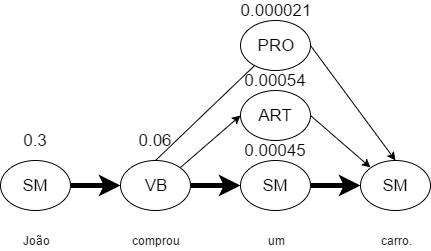
\includegraphics[height=180px]{imagens/markov2.png}
 \caption{Caminhos já decididos de classificação}
 \label{fig:markov2}
\end{figure}

Como visto, o método simbólico para resolver problemas de Processamento de
Linguagem Natural faz uso da criação de regras baseadas no conhecimento humano,
enquanto o método estatístico, decide através de cálculos probabilísticos
apoiados em estatísticas de um banco de dados para a resolução correta do
problema.


% Uma maneira de diferenciarmos os dois métodos é através do problema de
% ambiguidade. Por exemplo, nas frases:
% 
% ``João entrou no carro conversível de óculos novos.''. E ``João entrou no carro
% conversível de farol apagado.''.
% 
% Em ambas as frases, após a preposição ``de'' segue um substantivo masculino.
% Porém, cada uma das frases se refere a um substantivo diferente. A
% primeira se refere ao João, visto que não existe sentido em um carro ter óculos.
% Já a segunda se refere ao próprio carro, visto que não existe sentido em João
% ter faróis.
% 
% O método simbólico para resolver esse problema faz a criação de novas regras se
% baseadas no conhecimento humano para a solução de qual o significado da frase.
% Já o método estatístico, irá verificar qual a probabilidade de cada significado
% para cada frase através de análises similares decidindo através de metódos
% estatísticos qual o significado correto para cada frase
% \cite{jacksonmoulinier2007}.

\section{Métodos estatísticos e simbólicos aplicados na análise de sentimentos}
\label{cap:Classificadores}

%Para o \ac{NLP} e também para o campo de estatísticas, classificadores são
%algorítmos que identificam a qual categoria determinado item pertence. Essa
%classificação é feita a partir de dados já classificados corretamente, ou seja,
%um \textit{training set}.

\subsection{Naive Bayes}

O classificador Naive Bayes é um classificador baseado no teorema de Bayes com
independencia entre seus atributos.

O teorema de Bayes é representado da seguinte forma:

\[ P(c|d) = \frac{P(d|c) P(c)}{P(d)}  \]

Supondo que precisamos determinar se o carro que João comprou na frase ``João
comprou um Focus.'' é o modelo sedan ou hatch.
 
\begin{itemize}
  \item P(c$\vert$d) é a probabilidade de \textbf{d} pertencer a classe
  \textbf{c}. Ou seja, a probabilidade do carro Focus ser um sedan.
  \item P(d$\vert$c) é a probabilidade da classe \textbf{c} ser \textbf{d}. Ou
  seja, dentre todas as sedans, a probabilidade de um sedan ser
  um Focus.
  \item P(c) é a probabilidade da classe \textbf{c}. Ou seja, a frequência que
  sedans aparecem no nosso banco de dados.
  \item P(d) é a probabilidade de \textbf{d}. Ou seja, a frequência que Focus aparecem no nosso banco de dados.
\end{itemize}

Levando em consideração que temos o banco de dados representado pela tabela
abaixo:

\begin{table}[htb]
\centering
\label{123}
\begin{tabular}{|l|l|}
\hline
Carro  & Categoria \\ \hline
Focus  & Sedan     \\ \hline
Gol    & Hatch     \\ \hline
Focus  & Hatch     \\ \hline
Focus  & Sedan     \\ \hline
Focus  & Hatch     \\ \hline
Fox    & Hatch     \\ \hline
Fiesta & Hatch     \\ \hline
Cruze  & Sedan     \\ \hline
Focus  & Hatch     \\ \hline
\end{tabular} 
\caption{Tabela de Carro e Categoria.}
\end{table}

Probabilidade do Focus ser sedan:

\[ P(Sedan|Focus) = \frac{P(Focus|Sedan) P(Sedan)}{P(Focus)}  \]

\[ P(Sedan|Focus) = \frac{2/3 * 3/10}{5/10} = \frac{0,2}{0,5} = 0,4\]

Probabilidade do Focus ser um hatch:

\[ P(Hatch|Focus) = \frac{P(Focus|Hatch) P(Hatch)}{P(Focus)}  \]

\[ P(Hatch|Focus) = \frac{3/6 * 7/10}{5/10} = \frac{0,35}{0,5} = 0,7\]

No caso utilizado como exemplo, o Focus(Atributo ou \textit{Feature}) é um hatch
(Rótulo ou \textit{Label}).
Porém, caso tenhamos mais um atributo para utilizar na classificação o classificador Naive Bayes não
considera nenhuma dependência.
Como por exemplo a frase ``O carro era ano 2010 e tinha 2 portas'' com os
seguintes atributos:

\begin{table}[htb]
\centering
\begin{tabular}{|l|l|l|l|}
\hline
Carro  & Ano  & Portas & Categoria \\ \hline
Focus  & 2010 & 2      & Sedan     \\ \hline
Gol    & 2010 & 4      & Hatch     \\ \hline
Focus  & 2011 & 4      & Hatch     \\ \hline
Focus  & 2011 & 2      & Sedan     \\ \hline
Focus  & 2011 & 2      & Hatch     \\ \hline
Fox    & 2012 & 4      & Hatch     \\ \hline
Fiesta & 2012 & 2      & Hatch     \\ \hline
Cruze  & 2013 & 4      & Sedan     \\ \hline
Focus  & 2013 & 2      & Hatch     \\ \hline
\end{tabular}
\caption{Tabela de anos, carros, portas e categorias.}
\label{my-label}
\end{table}

O cálculo será feito da seguinte forma:

\[ P(d|c) = P(d_1|c) * P(d_2|c)* \ldots * P(d_n|c) \]

\[ P(Sedan|Focus) = P(Portas=2|Sedan) * P(Ano=2010|Sedan) \ldots * \]

\[ P(Sedan|Focus) = 2/3 * 1/3 \ldots * \]

Por assumir independência entre seus atributos, os valores obtidos nós cálculos
podem ser armazenados no banco de dados e reaproveitados. Por isso, sua
performance é considerada incrívelmente boa até mesmo para casos aonde temos forte dependência de
atributos \cite{domingos97naivebayes}.

%TODO EXEMPLO
\subsection{\textit{Maximum Entropy}}
O classificador \ac{MaxEnt} tem como
característica principal a preferência por modelos de dados uniformes sem efetuar nenhuma suposição injustificada.

Podemos utilizar um exemplo similar ao anterior para demonstrar a lógica do
classificador \ac{MaxEnt}. 
 
``João comprou um carro.''.

Supondo que temos que classificar o tipo de carro comprado em três categorias:

\begin{itemize}
  \item Hatch.
  \item Sedan.
  \item Cupê.
\end{itemize}

Podemos afirmar que:

\[ P(Hatch) + P (Sedan) + P(Cupe) = 1 \]

Como só temos essas três possibilidades de classificação no nosso
exemplo, o carro só pode ser classificado em uma dessas três possibilidades, ou
seja, a soma das três probabilidades deve ser 100\% ou 1 essa é a primeira
restrição ou \textit{constraint}. Abaixo duas tabelas que satisfazem essa
restrição:

\begin{table}[htb]
\centering
\begin{tabular}{|l|l|}
\hline
Tipo  & \%   \\ \hline
Sedan & 33\% \\ \hline
Hatch & 33\% \\ \hline
Cupê  & 33\% \\ \hline
 \end{tabular}
\caption{Tabela de Probabilidades A} 
\end{table}
\begin{table}[htb]
\centering
 \begin{tabular}{|l|l|}
\hline
Tipo  & \%   \\ \hline
Sedan & 50\% \\ \hline
Hatch & 50\% \\ \hline
Cupê  & 0\% \\ \hline
 \end{tabular}  
\caption{Tabela de Probabilidades B} 
\end{table}

Sem nenhum conhecimento prévio da distribuição desses carros, ou seja, a
quantidade de carros comprados por tipo, o classificador assume uma distribuição
uniforme das probabilidades, portanto, com maior entropia.

\begin{itemize}
  \item Hatch - 33\%.
  \item Sedan - 33\%.
  \item Cupê - 33\%.
\end{itemize}

Agora, supondo que a partir do nosso banco de dados conseguimos verificar que em
80\% dos casos o veículo comprado era um sedan ou hatch, temos uma nova
restrição:

\[ P(Hatch) + P (Sedan) = 0.8 \]

Podemos novamente ter n distribuições diferentes, porém a distribuição mais
uniforme que satisfaz as nossas duas restrições são:

\begin{itemize}
  \item Hatch - 40\%.
  \item Sedan - 40\%.
  \item Cupê - 30\%.
\end{itemize}

Esse é o princípio da Máxima Entropia utilizado nessa forma de classificação.
Primeiro é descoberta a frequência de cada atributo, depois é procurada a
distribuição que máximiza a entropia, ou seja, a mais uniforme.

%\subsection{Modelo Probabilístico}

%O seu modelo probabilístico para as probabilidades de observarmos o evento c
%quando d for verdadeiro:

%\[ P(c|d) := \frac{1}{Z(d)} exp (\Sigma_i\lambda_{i,c}F_{i,c}(d,c))\]





\subsection{\textit{VADER}}

O \ac{VADER} é um dicionário e classificador de sentimentos que se baseia em
regras, portanto, um método de classificação simbólico. Ele é especialmente
ajustado para funcionar em redes sociais aonde temos um contexto vago e pouca
quantidade de texto, nesse contexto, ele é extremamente eficaz, podendo se
comparar a classificação feita por humanos \cite{conf/icwsm/HuttoG14}.

Esse método faz uso de um dicionário que foi construído levando em consideração
gírias e emoticons utilizados em redes sociais. Neste dicionário as palavras
estão previamente associadas a uma polaridade de sentimento (positivo e
negativo) e intensidade em uma escala de -4 até +4, como por exemplo, a palavra
\textit{great} tem a intensidade de 3.1 e \textit{horrible} -2.5. Essa
associação foi construída utilizando o método de \textit{``wisdom of the
crowd''} aonde um grupo de pessoas atribuiu os valores para cada palavra ao
invés de somente uma pessoa especializada ou uma classificação automática
através de estatística.

Ele faz uso de cinco regras gerais:


\begin{itemize}
  \item Pontuação. O ponto de exclamação (!) aumenta a magnitude da
  intensidade sem modificar a orientação semântica. Como por exemplo,
  \textit{``This place is great!!!''} é mais intenso que \textit{``This place
  is great''}.
  \item Capitalização. Especificamente, uma palavra que é relevante para a
  análise de sentimentos, quando essa é escrita em letras maiúsculas, é
  aumentada a magnitude da intensidade do sentimento sem modificar a orientação
  semântica. Como por exemplo, na frase \textit{``This place is GREAT''}, temos
  a palavra \textit{``GREAT''} (Ótimo) que está relacionada com o sentimento
  positivo. Neste caso aonde ela está escrita em letras maiúsculas, ela é mais
  intensa que \textit{``This place is great''}.
  \item Advérbios intensificadores. Estes impactam a intensidade do sentimento
  aumentando ou diminuindo a intensidade do sentimento. Na frase \textit{``This
  place is extremelly good''} o advérbio \textit{extremelly} (extremamente)
  aumenta a intensidade do sentimento expresso pela frase (\textit{good} ou
  bom), enquanto na frase \textit{``This place is marginally good''}, a palavra
  \textit{``marginally'' ou marginalmente} acaba diminuindo a intensidade do
  sentimento expresso.
  \item A palavra \textit{``but''}. Essa palavra indica uma troca no sentimento
  da frase expressa aonde que o texto seguinte a ela expressa um sentimento mais
  dominante. Por exemplo, a frase \textit{``This place is great but today, the
  service was horrible''} convém um sentimento misto.
  \item Por fim, ao examinar as três palavras anteriores, o método consegue
  identificar 90\% dos casos aonde uma negação inverte a polaridade de um texto.
  Como por exemplo, na frase \textit{``This place isn't that great''}, a
  palavra \textit{great} demonstra um sentimento positivo, porém, ao analisar
  as três palavras anteriores \textit{``place isn't that''} encontramos uma
  negação, mudando o sentimento expresso da frase de positivo para negativo.
\end{itemize}


%\chapter{Frameworks}
\label{cap:Frameworks}

\section{Natural Language Toolkit}

O \ac{NLTK} é um \textit{Framework} para Python
criado em 2001 na Universidade de Pensilvânia. Ele contém mais de 50 dicionários
e modelos já treinados incluindo:

\begin{itemize}
  \item \textit{Sentiment Polarity Dataset Version 2.0} - Conjunto de dados já
  classificados que contém mais de 1000 filmes avaliados de forma positiva e
  1000 filmes avaliados de forma negativa.
  \item \textit{SentiWordNet} - Provém um dicionário com as palavras extraídas
  do WordNet já classificadas em positividade, negatividade e objetividade.
  \item \textit{VADER Sentiment Lexicon} - Dicionário especificamente ajustado
  para análise de sentimentos expressos em mídias sociais.
\end{itemize}


\subsection{Análise de Sentimentos}

Para a análise de sentimentos, o \ac{NLTK} já possui implementado os três
classificadores citados anteriormente, \textit{Naive Bayes},
\ac{MaxEnt} e também \ac{VADER}.

Podemos utilizar o classificador Naive Bayes a partir da classe

\textbf{nltk.classify.naivebayes.NaiveBayesClassifier} através dos seguintes métodos:

\begin{itemize}
  \item \textit{classify(featureset)} - Classifica a partir de um conjunto de
  atributos.
  \item \textit{most\_informative\_features(n=100)} - A partir de um
  classificador treinado, retorna os atributos mais relevantes.
  \item \textit{train(trainingset)} - Treina um classificador a partir de um \textit{training set}.
\end{itemize}

Podemos utilizar o classificador \ac{MaxEnt} a partir do módulo
\textbf{nltk.classify.maxent} através dos seguintes métodos:

\begin{itemize}
  \item \textit{train(train\_toks, algorithm=None, trace=3,
  encoding=None, labels=None, gaussian\_prior\_sigma=0, **cutoffs)} - Treina um
  classificador \ac{MaxEnt} a partir de um \textit{training set}.
  \begin{itemize}
    \item \textit{train\_toks} - \textit{Training set}.
  \item \textit{algorithm} - Algorítmo a ser usado para treinar o classificador. 
%   Pode receber: \textit{Generalized Iterative Scaling ('GIS')}, \textit{Improved
%   Iterative Scaling ('IIS')} ou LM-BFGS ('megam'). O algorítmo utilizado
%   por padrão é IIS.
  \item \textit{trace} - Nível de detalhe utilizado no log.
  \item \textit{encoding}
  \item \textit{labels} - Uma lista de possíveis rótulos, se nenhuma for
  especificada, todos os labels do \textit{training set} serão utilizados.
  \item \textit{gaussian\_prior\_sigma=0} - Somente utilizado no LM-BFGS.
  \item \textit{cutoffs} - Argumentos que especificam condições em que o
  processo será terminado.
  \end{itemize}
\item \textit{classify(featureset)} - Classifica a partir de um conjunto de
  atributos.
\item \textit{explain(featureset, columns=4)} - Mostra uma tabela demonstrando
os efetiso de cada atributo e como eles combinam para determinar a probabilidade
de cada rótulo.
\item \textit{show\_most\_informative\_features(n=10, show='all')} - A partir de
um classificador treinado, retorna os atributos mais relevantes.
\end{itemize}

Para utilização do \ac{VADER} é utilizada a classe
\textit{SentimentIntensityAnalyzer} do módulo \textit{vaderSentiment} através
do método \textit{polarity\_scores}. Este método recebe uma frase e retorna um
objeto contendo a intensidade positiva, neutra e negativa da frase.

O \textit{framework}
também contém um pacote contendo classes úteis para a análise de sentimentos
chamado de \textit{nltk.sentiment}. Nesse pacote temos os seguintes módulos:


\begin{itemize}
  \item Classe \textit{nltk.sentiment.sentiment\_analyzer.SentimentAnalyzer} -
  Ferramentas para facilitar e implementar análise de sentimentos,
  especialmente para demonstrações e ensino.
  \item Módulo \textit{nltk.sentiment.util} - Contém diversas classes de
  demonstrações e utilitários como conversão de \textit{json} para \textit{csv}.
\end{itemize}

\section{Stanford CoreNLP}

O Stanford CoreNLP é um conjunto de ferramentas escrito em Java para
processamento de linguagem natural. Dentre essas ferramentas, estão incluídos:
\textit{Part-of-Speech Tagging} ou classificação gramatical, reconhecimento de
entidade e análise de sentimentos. Também possui suporte a diversas linguas além
do inglês, como: árabe, chinês, francês, alemão e espanhol.

\subsection{Análise de Sentimentos}

A análise de sentimentos do Stanford CoreNLP é realizada através de um novo
modelo de rede neural construído em cima de estruturas gramaticais chamado de
\ac{RNTN}. Seu modelo é treinado a partir do \textit{Sentiment Treebank}, um
banco de dados que possui 215.154 orações distribuidas em 11.855 árvores de
frases com sentimentos já classificados.

\begin{figure}[htbp]
 \centering
 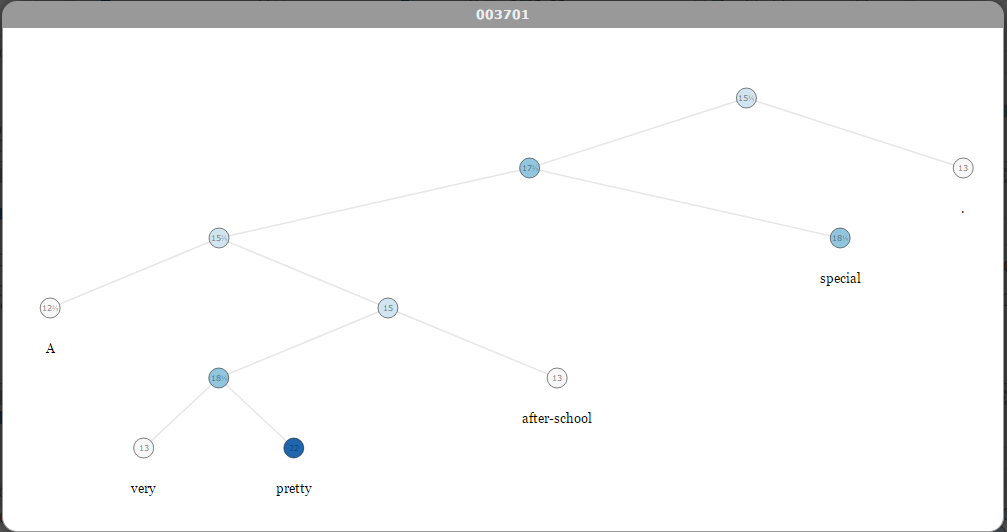
\includegraphics[height=225px]{imagens/corenlp.png}
 \caption{Frase já classificada disponível no Sentiment Treebank}
 \label{fig:corenlp}
\end{figure}

A sua utilização pode ser feita de diversas formas, como linha de comando,
através de um servidor \textit{web} e através de sua API java:


\begin{figure}[htbp]
 \centering
 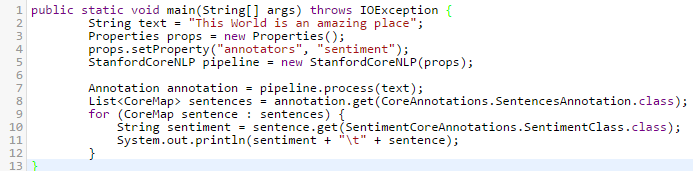
\includegraphics[height=120px]{imagens/corenlp1.png}
 \caption{Exemplo de implementação}
 \label{fig:corenlp}
\end{figure}

Como resultado, o console java irá imprimir que a frase é muito positiva ou
\textit{Very positive}.


\chapter{Criação de Base de Dados}
\label{cap:banco}
Este capítulo tem como objetivo descrever a rede social Reddit.
Após, são apresentados os tópicos que foram selecionados para a análise de
sentimentos. Por fim, é apresentada a ferramenta desenvolvida para a extração
dos comentários destes tópicos e para a criação da base.
\section{Rede Social Reddit}
\label{cap:Reddit}

O \textit{website} Reddit foi criado por Alexis Ohanian e Steve Huffman e teve
seu início em 2005 como um agregador de conteúdo e, atualmente, é o vigésimo terceiro \textit{website} mais acessado na
internet e o sétimo mais acessado nos Estados Unidos da América \cite{alexa}.
Os usuários do Reddit podem enviar \textit{links} com conteúdos externos
ao Reddit ou ainda mensagens de texto. A partir desse conteúdo, os seus
usuários podem votar para cima (\textit{upvote}) ou para baixo \textit{downvote},
influenciando na posição do conteúdo no \textit{website}. Além de votar no conteúdo, seus usuários podem enviar comentários como
forma de expressar sua opinião (Figura \ref{fig:reddit}).

\newpage

\begin{figure}[!htbp]
\centering

\includegraphics[height=300px]{imagens/reddit.png}
\caption{\textit{Website Reddit}:  As flechas demarcadas permitem efetuarmos
\textit{upvotes} ou \textit{downvotes}.}
\label{fig:reddit}
\end{figure}

O conteúdo do Reddit é distribuído em \textit{subreddits} que funcionam como
comunidades. Os usuários podem se inscrever nesses
\textit{subreddits}, recebendo as atualizações na sua página inicial, sendo
que dentre esses \textit{subreddits}, destacam-se:


\begin{itemize}
  \item \textit{/r/AskReddit}: esse \textit{subreddit} é utilizado para fazer
  perguntas gerais para outros usuários do Reddit. Esse \textit{subreddit}
  possui aproximadamente 16.941.540 inscritos.
  \item \textit{/r/worldnews}: esse \textit{subreddit} possui as notícias de
  todo o mundo, contando com aproximadamente 16.570.600 inscritos.
  \item \textit{/r/IAmA}: IAmA é um estilização de 'I am a' ('Eu sou um'):
  a partir desse \textit{subreddit} os usuários podem fazer perguntas ao criador
  de um determinado tópico. Esse \textit{subreddit} possui aproximadamente
  16.990.160 inscritos.
\end{itemize}

% Dentre esses \textit{subreddits} podemos destacar alguns dos tópicos mais
% acessados no ano de 2016:
% 
% \begin{itemize}
%   \item \textit{/r/IAmA} - \textit{We're NASA scientists \& exoplanet experts.
%   Ask us anything about today's announcement of seven Earth-size planets
%   orbiting TRAPPIST-1!} - Tópico de perguntas e respostas com cientistas da
%   NASA após a descoberta dos planetas que orbitavam a estrela TRAPPIST-1.
%   \item \textit{/r/IAmA} - \textit{I’m Bill Gates, co-chair of the Bill \&
%   Melinda Gates Foundation. Ask Me Anything.} - Tópico de perguntas e respostas com Bill Gates.
%   \item \textit{/r/worldnews} - \textit{Fidel Castro is dead at 90.} - Link para
%   anúncio da morte de Fidel Castro.
%   \item \textit{/r/AskReddit} - \textit{[Serious]South Koreans of Reddit, how
%   did they teach you about the existence of North Korea in School when you were
%   young?serious replies only} - Tópico perguntando para os usuários sul coreanos
%   como que foi ensinado para eles sobre a existência da Coreia do Norte.
% \end{itemize}

% A identificação de padrões de sentimentos expressos por determinados grupos
% dessa comunidade, se faz útil visto que a partir dessa avaliação é possível construir
% ferramentas que apoiam decisões tanto de um ponto de vista político, como por
% exemplo, entender qual é a opinião sobre um determinado assunto de um conjunto
% de eleitores, tanto quanto um ponto de vista de negócios, para entender qual a
% opinião dos consumidores de um produto, ou de seu competidor, a respeito de um
% determinado assunto.

\section{Extração de Dados}
\label{cap:Extracao}

Para a extração comentários do \textit{website} Reddit e para a criação da base
foi desenvolvido um \textit{crawler} ou robô de navegação. Esse robô foi
implementado na linguagem Java e tem como objetivo a navegação automática no
conteúdo do \textit{website} Reddit, extraindo os dados e comentários referentes a um
determinado tópico. Após, os dados são armazenados em banco de dados MySQL
\cite{Widenius:2002:MRM:560480}.
Na Figura \ref{fig:crawler} tem-se a arquitetura do \textit{software}
desenvolvido. O código deste encontra-se no CD em anexo.

\begin{figure}[htbp]
\centering
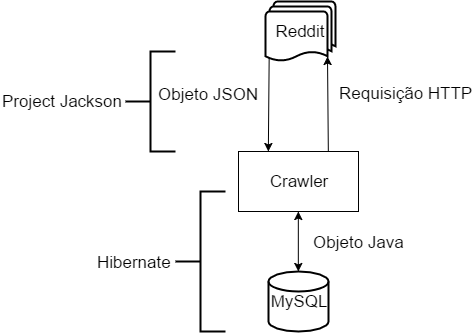
\includegraphics[height=225px]{imagens/arquitetura.png}
\caption{Arquitetura do \textit{Crawler}}
\label{fig:crawler}
\end{figure}

A partir de um \textit{link} para um tópico, o robô efetua uma busca e a
extração dos dados relacionados a esse tópico. Para tanto, foi utilizada a
\ac{API} do Reddit, onde, inicialmente envia-se uma requisição utilizando o
sufixo ``.json'' (Por exemplo:
\textit{\url{https://www.reddit.com/r/iama.json}}) e, a partir dessa requisição,
o \textit{website} retorna um objeto \ac{JSON}. Uma vez que o \ac{JSON}
retornado pelo \textit{website} possui 68 campos e que esses não se encontram
documentados, utilizou-se o \textit{website}
jsonschema2pojo\footnote{http://www.jsonschema2pojo.org/ - O \textit{website}
jsonschema2pojo tem como objetivo a conversão de um esquema \ac{JSON} em
\textit{Plain Old Java Objects}\ac{POJO}, permitindo o \textit{download} da classe para a utilização.} para converter o
JSON retornado em um \textit{Plain Old Java Objects} (\ac{POJO}).

Após, foi utilizado o \textit{framework} Hibernate
\cite{Iverson:2004:HJD:1044870} para a criação do banco de dados e para a
persistência dos dados. O Hibernate é um \textit{framework} de
mapeamento objeto-relacional que tem como objetivo representar tabelas do banco
de dados através de classes, ou seja, esse \textit{framework} tem como principal
característica a transformação das classes em Java para tabelas em um banco de dados relacional.
No caso deste trabalho, ele é responsável pela criação das tabelas \textit{RedditPost} e
\textit{RedditThread}, relacionadas, respectivamente, com os comentários e o
tópico em questão. 

\section{Tópicos Selecionados}

Para análise de sentimentos e para comparação dos resultados obtidos, foram
selecionados 15 tópicos, sendo que esses tópicos são os que
apresentam o maior número de comentários no último ano. Destaca-se que os 15
tópicos encontram-se distribuídos em diferentes assuntos, que são: cenário
político nacional, cenário político internacional e tópicos diversos:

No que diz respeito a tópicos relacionados com ao cenário político nacional, os
tópicos escolhidos foram:
\sloppy
\begin{itemize}
  \item
  \textit{Brazil Seeks To Copy U.S. Gun Culture ``to allow embattled
  citizens the right to defend themselves from
  criminals''}: esse tópico encontra-se disponível em 
  \url{https://www.reddit.com/r/worldnews/comments/36ny58/brazil_blogger_known_for_reporting_on_corruption/}
  e refere-se a intenção do Brasil em adotar a cultura de porte de armas dos
  Estados Unidos da América.
  \item
  \textit{Brazil descends into chaos as Olympics looms}: esse tópico encontra-se disponível em 
  \url{https://www.reddit.com/r/worldnews/comments/4bqcc3/brazil_descends_into_chaos_as_olympics_looms/}
  e refere-se ao caos ocorrido nas Olímpiadas de 2016 que foram realizadas no
  Brasil.
  \item
  \textit{Plane carrying Brazil Supreme Court judge crashes into sea}: esse tópico encontra-se disponível em
  \url{https://www.reddit.com/r/worldnews/comments/5oyz3b/plane_carrying_brazil_supreme_court_judge_crashes/}
  e refere-se a queda do avião no qual o ministro Teori Zavascki estava abordo.
  \item
  \textit{Brazil passes Internet governance Bill: Brazil has made history with
  the approval of a post-Snowden Bill which sets out principles, rights and
  guarantees for Internet users.}: esse tópico encontra-se disponível em
  \url{https://www.reddit.com/r/worldnews/comments/21f3as/brazil_passes_internet_governance_bill_brazil_has/}
  e refere-se a aprovação do Marco Civil da Internet.
  \item
  \textit{FIFA generated more than \$4 billion in sales from the 2014 World Cup,
  and is Giving Brazil \$100 Million After The Country Spent \$15 Billion On The
  World Cup}: esse tópico encontra-se disponível em
  \url{https://www.reddit.com/r/worldnews/comments/2t65ql/fifa_generated_more_than_4_billion_in_sales_from/}
  e refere-se a diferença entre o que foi gasto e o que foi arrecadado pelo
  Brasil na Copa do Mundo de 2014.
 
\end{itemize}

Já os tópicos escolhidos que se referem a política internacional são:
\begin{itemize}
  \item
  \textit{2.6 terabyte leak of Panamanian shell company data reveals "how a
  global industry led by major banks, legal firms, and asset management companies
  secretly manages the estates of politicians, Fifa officials, fraudsters and
  drug smugglers, celebrities and professional
  athletes."}.: esse tópico encontra-se disponível em
  \url{https://www.reddit.com/r/worldnews/comments/4d75i7/26_terabyte_leak_of_panamanian_shell_company_data/}
  e se refere ao vazamento dos documentos confidenciais de uma
  sociedade de advogados panamenha. Esses documentos apresentam informações
  detalhadas de empresas localizadas em paraísos fiscais.
  \item
  \textit{Fidel Castro is dead at
  90.}: esse tópico encontra-se disponível em
  \url{https://www.reddit.com/r/worldnews/comments/5exz2e/fidel_castro_is_dead_at_90/}
  e se refere a morte do presidente de Cuba, Fidel Castro.
  
  \item
  \textit{Donald Trump to strip all funding from State Dept team promoting
  women's rights around the world - Leaked plan comes as First Daughter Ivanka
  defends her father's record with women}: esse tópico encontra-se disponível em
  \url{https://www.reddit.com/r/worldnews/comments/67ivae/donald_trump_to_strip_all_funding_from_state_dept/}
  e refere-se a decisão do presidente dos Estados Unidos da América, Donald
  Trump, em remover fundos de promoção ao direito das mulheres.
  
  \item
  \textit{Manchester Arena 'explosions': Two loud bangs heard at MEN Arena}:
  esse tópico encontra-se disponível em
  \url{https://www.reddit.com/r/worldnews/comments/6cqdye/manchester_arena_explosions_two_loud_bangs_heard/}
  e refere-se ao atentado terrorista ocorrido na Manchester Arena (Inglaterra)
  em 23 de Maio de 2017.
  
  \item
  \textit{Sweden asks the U.S. to explain Trump comment on
  Sweden}: esse tópico encontra-se disponível em
  \url{https://www.reddit.com/r/worldnews/comments/5uzetf/sweden_asks_the_us_to_explain_trump_comment_on/}
  e se refere aos comentários feitos do presidente dos Estados Unidos da
  América, Donald Trump, sobre a Suécia.
  
  \item\textit{“Canada will welcome you,” Trudeau invites refugees as Trump bans
  them}: esse tópico encontra-se disponível em
  \url{https://www.reddit.com/r/worldnews/comments/5qqa51/canada_will_welcome_you_trudeau_invites_refugees/}
  e refere-se a declaração do primeiro ministro canadense sobre decisão de
  receber refugiados. Neste declaração, o primeiro ministro canadense afirma que
  os refugiados serão bem-vindos no Canadá.
\end{itemize}

Por fim, os tópicos selecionados que abordam assuntos diversos foram:
\begin{itemize}
  \item
  \textit{I’m Bill Gates, co-chair of the Bill \& Melinda Gates Foundation. Ask
  Me Anything.}: esse tópico encontra-se disponível em
  \url{https://www.reddit.com/r/IAmA/comments/5whpqs/im_bill_gates_cochair_of_the_bill_melinda_gates/}
  e apresenta as respostas de perguntas que foram feitas ao fundador
  da Microsoft, Bill Gates.
  \item
  \textit{Hey, it's Lars from Metallica. AMA}: esse tópico encontra-se disponível em
  \url{https://www.reddit.com/r/IAmA/comments/1wl9ic/hey_its_lars_from_metallica_ama/}.
  Esse tópico apresenta as respostas de perguntas que foram realizadas ao
  vocalista da banda de rock Metallica, James Hetfield.
  \item
  \textit{I'm the CEO of Renault and Nissan and we're making autonomous driving
  vehicles happen by 2020. Ask me anything!}: esse tópico encontra-se disponível em
  \url{https://www.reddit.com/r/IAmA/comments/2s7obx/im_the_ceo_of_renault_and_nissan_and_were_making/}
  e refere-se as respostas às perguntas realizadas ao diretor executivo da Renault e Nissan,
  Carlos Ghosn.
  
  \item
  \textit{I am Julian Assange founder of WikiLeaks -- Ask Me Anything}: esse
  tópico encontra-se disponível em
  \url{https://www.reddit.com/r/IAmA/comments/5n58sm/i_am_julian_assange_founder_of_wikileaks_ask_me/}
  e refere-se as respostas às perguntas realizadas ao Julian Assange, fundador do
  \textit{WikiLeaks}.
  
\end{itemize}


Destaca-se que para a criação da base de dados, somente foram extraídos
comentários em resposta ao tópico em questão, comentários em resposta a outros
comentários foram desconsiderados, uma vez que esses podem não estar diretamente
relacionados ao tópico em questão, tornando inválida ou prejudicando a análise de sentimento.


\chapter{Conclusão Parcial}
\label{cap:conclusao}
A \ac{NLP} tem como objetivo a análise de linguagem natural, seja
essa escrita ou falada. Dentre diversas tarefas que ela executa, tem-se a
análise de sentimentos, a qual recebeu destaque nos últimos anos devido ao fato das pessoas cada vez se comunicarem através de redes sociais,
gerando um grande volume de dados. A análise e quantificação da opinião expressa por esses dados, seja
por fins políticos, comerciais ou quaisquer outros, se torna díficil devido a
essa grande quantidade de dados.

Observou-se que os métodos mais utilizados para análise de sentimentos são o
Método de Naive Bayes (estatístico) e o Método de \ac{VADER} (simbólico). Dentre
estes, optou-se pela utilização do método de \ac{VADER}, uma vez que de acordo
com a literatura, esse apresenta um desempenho superior ao método de Naive
Bayes. De fato, esse mostrou-se superior na análise de sentimentos nas avaliações de
produtos da Amazon, editoriais do New York Times e mais importante, na análise
de \textit{Tweets} da rede social Twitter \cite{SentimentinSocialMedia}. A
justificativa para isso, se dá ao fato de métodos estatísticos necessitarem de um \textit{training set}
especializado para obter resultados similares ou superiores aos métodos
simbólicos. 

Além disso, optou-se pela utilização do método de \ac{VADER}, devido
ao fato deste não necessitar da criação de um \textit{training set} específico
para a análise de sentimentos. A necessidade da criação de um \textit{training
set} específico para cada tema inviabilizaria o desenvolvimento deste trabalho,
uma vez que neste serão analisados 15 tópicos com temas distintos. Para
implementação do método \ac{VADER} optou-se pela biblioteca \ac{NLTK}. A
utilização da biblioteca \ac{NLTK} permitirá a utilização futura de outros
métodos de \ac{NLP}, bem como um estudo da performance do Método de \ac{VADER} e esses outros métodos.
 
Por fim, se fez necessária a criação de uma base de dados para armazenar os
tópicos e os comentários disponibilizados pela rede social Reddit. Para isso,
foi desenvolvido um \textit{crawler} (robô) que é responsável por extrair os
comentários relacionados a um tópico na rede social Reddit e armazenar em um
banco de dados MySQL. Esse robô foi desenvolvido na linguagem Java e utiliza a
API da rede social Reddit para extrair as informações de um tópico. Após, ele
utiliza o \textit{framework} Hibernate para armazenar os dados extraídos na
base de dados MySQL.

Na segunda etapa deste trabalho, será utilizado o \textit{framework} \ac{NLTK}
para efetuar a análise de sentimento sobre a base de dados criada. Essa análise
tem como principal objetivo identificar padrões de sentimentos entre
usuários e comunidades da rede Reddit.

\section{Atividades e Cronograma}

Na Tabela \ref{tab:tcc1} tem-se o cronongrama das atividades realizadas durante
o TCC I. Como pode ser observado, todas as tarefas programadas foram
realizadas.
\begin{enumerate}
\item Estudo de algoritmos para o processamento de texto e também análise de
sentimentos.
\item Análise das ferramentas já existentes.
\item Análise da API do Reddit.
\item Construção de um software para extração dos dados da API.
\item Extração e criação da base de dados.
\item Redação da monografia TCC I.
\item Apresentação TCC I.
\end{enumerate}

\renewcommand{\arraystretch}{2}
\newcolumntype{Y}{>{\centering\arraybackslash}X}
\begin{table}[!htb]
\begin{tabularx}{0.9\textwidth}{Y|Y|Y|Y|Y|Y|Y|Y|Y|Y|Y|}
& \multicolumn{2}{|c|}{Mar} & \multicolumn{2}{|c|}{Abr} &
\multicolumn{2}{|c|}{Mai} & \multicolumn{2}{|c|}{Jun} &
\multicolumn{2}{|c|}{Jul}
\\
\midrule
1 & \cellcolor{black!80} & \cellcolor{black!80} & & & & & & & & \\
2 &  & \cellcolor{black!80} & \cellcolor{black!80} & & & & & & &\\
3 &  &  &  & \cellcolor{black!80} & & & & & &\\
4 &  &  &  &  & \cellcolor{black!80} & & & &  &\\
5 &  &  &  &  &  & \cellcolor{black!80} & \cellcolor{black!80} & & &\\
6 &  & \cellcolor{black!80}  & \cellcolor{black!80}  &  \cellcolor{black!80} & 
\cellcolor{black!80} & \cellcolor{black!80} & \cellcolor{black!80} & \cellcolor{black!80} &  &\\
7 &  &  &  &  &  & & & & \cellcolor{black!80} &\\
\end{tabularx}

\caption{Cronograma do TCC I.}
\label{tab:tcc1}
\end{table}

Já na Tabela \ref{tab:tcc2} tem-se as atividades a serem desenvolvidas no TCC
II:

\begin{enumerate}
\item Implementação do software de Processamento de Linguagem Natural para a
análise de sentimentos na base de dados criada.
\item Análise dos resultados obtidos.
\item Redação da monografia TCC II.
\item Apresentação do TCC II.
\end{enumerate}

\newcolumntype{Y}{>{\centering\arraybackslash}X}
\begin{table}[!htb]
\begin{tabularx}{0.9\textwidth}{Y|Y|Y|Y|Y|Y|Y|Y|Y|Y|Y|}
& \multicolumn{2}{|c|}{Ago} & \multicolumn{2}{|c|}{Set} &
\multicolumn{2}{|c|}{Out} & \multicolumn{2}{|c|}{Nov} &
\multicolumn{2}{|c|}{Dez}
\\
\midrule
1 & \cellcolor{black!80} & \cellcolor{black!80} & \cellcolor{black!80} &
\cellcolor{black!80} & & & & & & \\
2 &  & & & \cellcolor{black!80} & \cellcolor{black!80} & \cellcolor{black!80} &
& & &\\
3 &  & \cellcolor{black!80} & \cellcolor{black!80} & \cellcolor{black!80} &
\cellcolor{black!80} & \cellcolor{black!80} & \cellcolor{black!80}
& \cellcolor{black!80} & &\\
4 &  &  &  &  &  & & & & \cellcolor{black!80} &\\
\end{tabularx}

\caption{Cronograma do TCC II.}
\label{tab:tcc2}
\end{table}

% No Capítulo \ref{cap:Processamento} foram introduzidos dois tipos de métodos
% distintos para o \ac{NLP}, métodos simbólicos e
% métodos estatísticos, os quais foram estudados para a análise de sentimentos
% através do Capítulo \ref{cap:Classificadores}.
% 
% Através do Capítulo \ref{cap:Classificadores}, foram comparados um método
% simbólico e outro método estatístico a fim de se determinar qual apresenta melhor performance na análise de sentimentos
% aplicada em uma rede social, sendo que a literatura apontou que o método mais
% assertivo é o método \ac{VADER}, o qual está disponível através do
% \textit{framework} \ac{NLTK}.
% 
% Já no Capítulo \ref{cap:banco}, foi apresentada como funciona a rede social
% Reddit, os tópicos selecionados para a análise de sentimentos, e por fim foi
% apresentado a forma na qual esses tópicos serão extraídos para população da base
% de dados.
% 
% A partir das informações demonstradas através deste, deverá ser possível criar
% um \textit{software} que efetue a análise de dados utilizando o \ac{VADER},
% através do \textit{framework} \ac{NLTK}, aplicada nos tópicos demonstrados no
% Capítulo \ref{cap:banco}.



%\chapter{Criação de Base de Dados}
\label{cap:banco}
Este capítulo tem como objetivo descrever a rede social Reddit.
Após, são apresentados os tópicos que foram selecionados para a análise de
sentimentos. Por fim, é apresentada a ferramenta desenvolvida para a extração
dos comentários destes tópicos e para a criação da base.
\section{Rede Social Reddit}
\label{cap:Reddit}

O \textit{website} Reddit foi criado por Alexis Ohanian e Steve Huffman e teve
seu início em 2005 como um agregador de conteúdo e, atualmente, é o vigésimo terceiro \textit{website} mais acessado na
internet e o sétimo mais acessado nos Estados Unidos da América \cite{alexa}.
Os usuários do Reddit podem enviar \textit{links} com conteúdos externos
ao Reddit ou ainda mensagens de texto. A partir desse conteúdo, os seus
usuários podem votar para cima (\textit{upvote}) ou para baixo \textit{downvote},
influenciando na posição do conteúdo no \textit{website}. Além de votar no conteúdo, seus usuários podem enviar comentários como
forma de expressar sua opinião (Figura \ref{fig:reddit}).


\begin{figure}[!htbp]
\centering

\includegraphics[height=300px]{imagens/reddit.png}
\caption{\textit{Website Reddit}:  As flechas demarcadas permitem efetuarmos
\textit{upvotes} ou \textit{downvotes}.}
\label{fig:reddit}
\end{figure}

O conteúdo do Reddit é distribuído em \textit{subreddits} que funcionam como
comunidades. Os usuários podem se inscrever nesses
\textit{subreddits}, recebendo as atualizações na sua página inicial, sendo
que dentre esses \textit{subreddits}, destacam-se:


\begin{itemize}
  \item \textit{/r/AskReddit}: esse \textit{subreddit} é utilizado para fazer
  perguntas gerais para outros usuários do Reddit. Esse \textit{subreddit}
  possui aproximadamente 16.941.540 inscritos.
  \item \textit{/r/worldnews}: esse \textit{subreddit} possui as notícias de
  todo o mundo, contando com aproximadamente 16.570.600 inscritos.
  \item \textit{/r/IAmA}: IAmA é um estilização de 'I am a' ('Eu sou um'):
  a partir desse \textit{subreddit} os usuários podem fazer perguntas ao criador
  de um determinado tópico. Esse \textit{subreddit} possui aproximadamente
  16.990.160 inscritos.
\end{itemize}

% Dentre esses \textit{subreddits} podemos destacar alguns dos tópicos mais
% acessados no ano de 2016:
% 
% \begin{itemize}
%   \item \textit{/r/IAmA} - \textit{We're NASA scientists \& exoplanet experts.
%   Ask us anything about today's announcement of seven Earth-size planets
%   orbiting TRAPPIST-1!} - Tópico de perguntas e respostas com cientistas da
%   NASA após a descoberta dos planetas que orbitavam a estrela TRAPPIST-1.
%   \item \textit{/r/IAmA} - \textit{I’m Bill Gates, co-chair of the Bill \&
%   Melinda Gates Foundation. Ask Me Anything.} - Tópico de perguntas e respostas com Bill Gates.
%   \item \textit{/r/worldnews} - \textit{Fidel Castro is dead at 90.} - Link para
%   anúncio da morte de Fidel Castro.
%   \item \textit{/r/AskReddit} - \textit{[Serious]South Koreans of Reddit, how
%   did they teach you about the existence of North Korea in School when you were
%   young?serious replies only} - Tópico perguntando para os usuários sul coreanos
%   como que foi ensinado para eles sobre a existência da Coreia do Norte.
% \end{itemize}

% A identificação de padrões de sentimentos expressos por determinados grupos
% dessa comunidade, se faz útil visto que a partir dessa avaliação é possível construir
% ferramentas que apoiam decisões tanto de um ponto de vista político, como por
% exemplo, entender qual é a opinião sobre um determinado assunto de um conjunto
% de eleitores, tanto quanto um ponto de vista de negócios, para entender qual a
% opinião dos consumidores de um produto, ou de seu competidor, a respeito de um
% determinado assunto.

\section{Extração de Dados}
\label{cap:Extracao}

Para a extração comentários do \textit{website} Reddit e para a criação da base
foi desenvolvido um \textit{crawler} ou robô de navegação. Esse robô foi
implementado na linguagem Java e tem como objetivo a navegação automática no
conteúdo do \textit{website} Reddit, extraindo os dados e comentários referentes a um
determinado tópico. Após, os dados são armazenados em uma base de dados criada
em um banco de dados MySQL \cite{Widenius:2002:MRM:560480}.
Na Figura \ref{fig:crawler} tem-se a arquitetura do \textit{software}
desenvolvido. O código deste encontra-se no CD em anexo.

\begin{figure}[htbp]
\centering
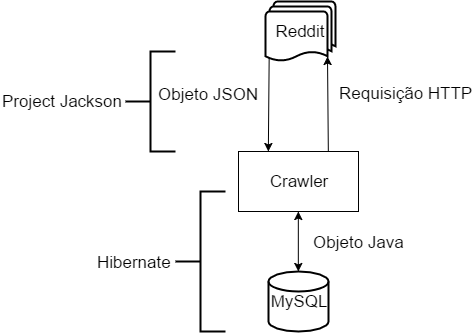
\includegraphics[height=225px]{imagens/arquitetura.png}
\caption{Arquitetura do \textit{Crawler}}
\label{fig:crawler}
\end{figure}

A partir de um \textit{link} para um tópico, o robô efetua uma busca e a
extração dos dados relacionados a esse tópico. Para tanto, foi utilizada a
\ac{API} do Reddit, onde, inicialmente envia-se uma requisição utilizando o
sufixo ``.json'' (Por exemplo:
\textit{\url{https://www.reddit.com/r/iama.json}}) e, a partir dessa requisição,
o \textit{website} retorna um objeto \ac{JSON}. Uma vez que o \ac{JSON}
retornado pelo \textit{website} possui 68 campos e que esses não se encontram
documentados, utilizou-se o \textit{website}
\textit{jsonschema2pojo}\footnote{http://www.jsonschema2pojo.org/ - O
\textit{website} jsonschema2pojo tem como objetivo a conversão de um esquema \ac{JSON} em
\textit{Plain Old Java Objects}\ac{POJO}, permitindo o \textit{download} da classe para a utilização.} para converter o
JSON retornado em um \textit{Plain Old Java Objects} (\ac{POJO}).

Após, foi utilizado o \textit{framework} Hibernate
\cite{Iverson:2004:HJD:1044870} para a criação do banco de dados e para a
persistência dos dados. O Hibernate é um \textit{framework} de
mapeamento objeto-relacional que tem como objetivo representar as tabelas de um
banco de dados através de classes, ou seja, esse \textit{framework} tem como principal
característica a transformação das classes em Java em tabelas em um banco de
dados relacional.
No caso deste trabalho, ele é responsável pela criação das tabelas \textit{RedditPost} e
\textit{RedditThread}, relacionadas, respectivamente, com os comentários e o
tópico em questão. 

\section{Validação da Implementação}

Após a extração dos dados, com o objetivo de validar a implementação
do método \ac{VADER}, foi selecionado o tópico:
\textit{``Canada will welcome you, Trudeau invites refugees as Trump bans
them''.}
A partir desse tópico, foram extraídos todos os comentários, que foram avaliados
de forma manual. Após, esses comentários foram processados através da ferramenta
\ac{NLTK}, obtendo uma assertividade de 56\%.

Destaca-se que uma grande parte dos comentários que foram identificados de forma
incorreta, apresentam a irônia como característica, como por exemplo, o
comentário \textit{``lol Good Luck Canada''}. A identificação da ironia através
da leitura textual se faz difícil até mesmo para um ser-humano, uma vez que o
texto pode não apresentar sinais de humor. A ironia para a análise de sentimentos é considerado
um tópico problemático sendo alvo de diversos estudos \cite{DBLP:conf/lrec/StranisciBFP16}.

Já para outros comentários que foram identificados de forma incorreta
observa-se que o sentimento expresso não no encontrava em dicionário de
sentimentos padrão do \ac{VADER}. De forma a minimizar este problema, foi
utilizado o método de Propagação Dupla, que possui como principal objetivo
adicionar novas palavras ao dicionário \cite{Qiu:2011:OWE:1970420.1970422}.

\section{Método de Propagação Dupla}

O método de Propagação Dupla, proposto por Qiu
\cite{Qiu:2011:OWE:1970420.1970422}, apresenta como objetivo resolver dois
problemas do \ac{NLP}, que são a expansão do dicionário e também a extração de
alvos de um comentário. Os \textit{``Opinion targets"} ou alvos de opinião, são
palavras as quais sentimentos se referem. Por exemplo, na frase ``Essa
música é muito boa", a palavra ``boa'' demonstra o sentimento do autor com relação a
``música'', tornando assim, a palavra música um alvo de opinião. 

A extração dos alvos é necessária pois em algumas frases
podemos ter opiniões sobre diferentes alvos. Além disso, podemos
ter opiniões diferentes sobre diferentes características de um alvo. Por
exemplo, na frase ``Este celular é muito bom, porém a bateria dele é péssima", tem-se que o produto em si é bom, porém, a opinião sobre a bateria dele é negativa. De
forma, a resolver esses problemas, novas palavras e alvos são adicionados ao
dicionário a partir da execução das quatro tarefas que serão descritas na
próxima seção.

\subsection{Adição de Palavras e Alvos ao Dicionário}

A \textbf{primeira tarefa}, é dividida em duas regras, sendo que a primeira
consiste na extração de alvos a partir de palavras que expressam sentimentos e
que já são conhecidas. Ou seja, são verificadas todas as palavras das quais a palavra que
expressa sentimentos depende. Caso essa palavra seja um substantivo, ela será
extraída e adicionada na lista de alvos de sentimentos. Por exemplo na frase \textit{``We have a great president''} a palavra \textit{``great''} depende de \textit{``president''}, que é um substantivo. Neste caso, a palavra \textit{``president''} será adicionada a
lista de alvos de sentimentos.

\[\textit{We have a } \underbrace{\textit{great president.}}_\text{president
\textrightarrow \text{ great}}\]

A segunda regra da primeira tarefa,
consiste em verificar se uma palavra que expressa sentimentos é dependente de
uma segunda palavra que depende de um substantivo.
Por exemplo, na frase \textit{``Trump is a great president.''} a palavra
\textit{``great''} depende da palavra \textit{``is''} que por sua vez depende da
palavra \textit{``president''} que é um substantivo. Neste caso, a palavra
\textit{``president''} será adicionada a lista de palavras que são alvos de sentimentos.

\[\textit{Trump} \underbrace{\textit{is a great president.}}_\text{president
\textrightarrow \text{ is} \textrightarrow \text{ great}}\]

A \textbf{segunda tarefa} é a extração de novas palavras que expressam
sentimentos. Para isso, são utilizadas duas regras. Na primeira regra, é
verificada se a frase possui alguma palavra que se encontra na lista de alvos de
sentimentos, em caso positivo, é verificado se essa palavra possui algum dependente que seja um adjetivo. Por exemplo, na frase \textit{``Trump is a witty president.''}, a palavra \textit{``president''} foi
extraída na tarefa anterior, porém, a palavra \textit{``witty''} ainda não se
encontra no dicionário de sentimentos.
Desta forma, a palavra \textit{``witty''} será acrescida ao
dicionário de sentimentos uma vez que essa palavra é um adjetivo e que ainda não
existe no dicionário.


\[\textit{We have a } \underbrace{\textit{witty president.}}_\text{president
\textrightarrow \text{ witty}}\]

A segunda regra da tarefa dois
consiste em verificar se uma palavra alvo possui um dependente, que por sua vez
possui um adjetivo como dependente. Por exemplo, na frase
\textit{``Trump is a witty president.''} a palavra \textit{``witty''}, que é um
adjetivo, depende de \textit{``is''} que por sua vez depende de
\textit{``president''}. Neste caso, a palavra \textit{``witty''}
será acrescida ao dicionário de sentimentos uma vez que essa é um adjetivo que
não existe ainda no dicionário.

\[\textit{Trump} \underbrace{\textit{is a witty president.}}_\text{president
\textrightarrow \text{ is} \textrightarrow \text{ witty}}\]

A \textbf{terceira tarefa} consiste na extração de palavras alvo a partir de
palavras alvo que já se encontram na lista de alvos. A primeira regra desta
tarefa verifica se a frase possui alguma palavra na lista de alvos, e verifica se essa possui alguma
conjunção. Em caso positivo, a palavra após a conjunção é adicionada na lista
de alvos. Por exemplo, na frase \textit{``We have a great president and
leader."}, a palavra \textit{``president''} que foi extraída através
da primeira tarefa, possui a conjunção \textit{``and''} que a relaciona com a
palavra \textit{``leader''}, a qual não consta na lista de alvos. Neste
caso, a palavra \textit{``leader''} será adicionada a lista de alvos.


\[\textit{We have a great} \underbrace{\textit{president and
leader.}}_\text{president \textrightarrow \text{ and} \textrightarrow \text{
leader}}\]

A segunda regra da terceira tarefa verifica se dois substantivos
possuem uma palavra dependente em comum. No caso de um desses substantivos ser
uma palavra alvo, o outro também é adicionado na lista. Por exemplo, na frase
\textit{``Trump is a great president.''}, a palavra \textit{``president''} que
foi extraída através da primeira tarefa possui a palavra \textit{``is''} como
dependente, bem como a palavra ``Trump'' também possui a palavra \textit{``is''}
como dependente. Desta forma, a palavra \textit{``Trump''} será adicionada a
lista de alvos.

\[\underbrace{\textit{Trump is a great president.}}_\text{Trump
\textrightarrow \text{ is} \textleftarrow \text{ president}}\]



A \textbf{quarta tarefa} tem como objetivo a extração de novas opiniões a partir
de adjetivos já extraídos. A primeira regra desta tarefa, efetua a extração através
das conjunções presentes no texto. Por exemplo, para a frase \textit{``Trump is
witty and clever.''}, a palavra \textit{``witty''} possui uma conjunção
(\textit{``and''}), que a relaciona com a palavra \textit{``clever''}. Neste
caso, a palavra \textit{``clever''} será adicionada ao dicionário.

\[\textit{Trump} \underbrace{\textit{is witty and clever.}}_\text{witty
\textleftarrow \text{ and} \textrightarrow \text{ clever}}\]


A segunda da quarta tarefa, consiste em verificar-se dois adjetivos
dependem de uma mesma palavra. Se uma destas palavras pertence ao dicionário de
sentimentos, a outra também será adicionada na lista. Por exemplo, na frase
\textit{``Trump is witty, clever''}, ambas as palavras \textit{``witty''} e
\textit{``clever''} dependem de \textit{``Trump''}. Neste caso, será extraída a
palavra \textit{``clever''} e adicionada ao dicionário.

\[\textit{Trump} \underbrace{\textit{is witty, clever.}}_\text{witty
\textleftarrow \text{ Trump} \textrightarrow \text{ clever}}\]

Por fim, é verificado se as listas de alvos ou sentimentos sofreram
alterações, ou seja, foram adicionadas novas palavras a essas listas. Em caso
positivo, as quatro tarefas serão executadas até que nenhuma palavra seja acrescentada a uma das listas.

\subsection{Atribuição de Pontuação às Novas Palavras}

Após a execução das quatro tarefas, se faz necessário definir a
pontuação relativa a polaridade do sentimento expresso pelas novas palavras
identificadas através do Método de Propagação Dupla para sua posterior
utilização através do método \ac{VADER}.

Essa atribuição é realizada da seguinte forma, para as palavras extraídas
através da quarta tarefa, é utilizada a mesma pontuação da palavra relacionada a
essa nova palavra. Por exemplo, para a frase \textit{``Trump is
witty and clever.''}, a palavra \textit{``witty''} possui uma conjunção
(\textit{``and''}), que a relaciona com a palavra \textit{``clever''}. Neste
caso, a palavra \textit{``clever''} terá a mesma pontuação da palavra
\textit{``witty''}.

Para a pontuação das palavras extraídas na tarefa dois, é realizado o seguinte
processo, na extração do alvo é atribuído a este alvo a mesma pontuação do
sentimento relacionado com ele. Por exemplo, na frase \textit{``We have a great
president''}, a palavra \textit{``president''} será adicionada a lista de alvos
de sentimentos com a mesma pontuação de \textit{``great''}, a qual está
relacionada. Após, essa pontuação é atribuída a palavra extraída na tarefa dois.
Por exemplo, no comentário \textit{``This president is witty.''}, na segunda
tarefa, a palavra \textit{``witty''}, que foi extraída através de
\textit{``president''}, irá receber a mesma pontuação da palavra \textit{``great''}.


Como visto, para utilização do método de Propagação Dupla, é necessário um
conjunto de textos para que sejam executadas as quatro tarefas. Segundo Qiu
\cite{Qiu:2011:OWE:1970420.1970422}, como as palavras tem diferentes
significados em diferentes contextos, é recomendado que este conjunto de textos
pertença ao mesmo contexto que está sendo efetuada a análise de sentimentos. Por
exemplo, ao utilizar um conjunto de dados sobre notícias gerais, pode-se
determinar que a palavra \textit{``gucci''} é uma gíria similar a palavra
\textit{``good''}. Porém, o uso dessa palavra em comentários de roupas
apresenta um outro contexto uma vez que se refere a uma marca de roupas.

A fim de se determinar o
melhor conjunto de textos para utilização do método, foram utilizados dois
conjuntos de dados de testes. No primeiro conjunto de textos, considerou-se
comentários de um mesmo usuário, desta forma, foram extraídos os 1000
comentários mais recentes dos usuários que comentaram no tópico \textit{``Canada will welcome
you,” Trudeau invites refugees as Trump bans them}, totalizando %TODO% 
comentários. Para o segundo
conjunto de textos, foram considerados comentários de usuários em tópicos
que apresentam o mesmo tema. Nesta avaliação, foram utilizados os seguintes
comentários:

\begin{itemize}
  \item
  \textit{Donald Trump to strip all funding from State Dept team promoting
  women's rights around the world - Leaked plan comes as First Daughter Ivanka
  defends her father's record with women}: esse tópico contém 9246
  comentários e encontra-se disponível em
  \url{https://www.reddit.com/r/worldnews/comments/67ivae/donald_trump_to_strip_all_funding_from_state_dept/}
  e refere-se a decisão do presidente dos Estados Unidos da América, Donald
  Trump, em remover fundos de promoção ao direito das mulheres.  
  \item
  \textit{Sweden asks the U.S. to explain Trump comment on
  Sweden}: esse tópico contém 10927
  comentários e encontra-se disponível em
  \url{https://www.reddit.com/r/worldnews/comments/5uzetf/sweden_asks_the_us_to_explain_trump_comment_on/}
  e se refere aos comentários feitos do presidente dos Estados Unidos da
  América, Donald Trump, sobre a Suécia.
  
  \item\textit{“Canada will welcome you,” Trudeau invites refugees as Trump bans
  them}: esse tópico contém 9113
  comentários e encontra-se disponível em
  \url{https://www.reddit.com/r/worldnews/comments/5qqa51/canada_will_welcome_you_trudeau_invites_refugees/}
  e refere-se a declaração do primeiro ministro canadense sobre decisão de
  receber refugiados. Neste declaração, o primeiro ministro canadense afirma que
  os refugiados serão bem-vindos no Canadá.
\end{itemize}
 
Após a utilização do Método de Propagação Dupla, utilizando os dois conjuntos
de textos e a avaliação dos comentários foram
obtidos os seguintes resultados a partir do tópico \textit{``Canada will welcome
you,” Trudeau invites refugees as Trump bans them}:
\begin{itemize}
  \item 58\% de assertividade na utilização do dicionário padrão.
  \item 59\% de assertividade na utilização do dicionário padrão com palavras
  extraídas a partir de comentários de um mesmo usuário.
  \item 62\% de assertividade na utilização do dicionário padrão com palavras
  extraídas a partir de comentários de um mesmo tema.
\end{itemize}
 
Destaca-se que mesmo com o aumento na assertividade com a utilização de
comentários de tópicos do mesmo domínio, os comentários que não foram
identificados de forma correta são comentários como: \textit{"...These
laws are not "racist", morons keep hysterically throwing that word around and
its losing all meaning..."}, aonde que o sentimento expresso é negativo, porém,
a pessoa expressa um sentimento a favor da notícia em questão. 

Para a solução deste problema, são extraídos somente os sentimentos relacionados
a uma palavra alvo. Por exemplo, no tópico \textit{``Canada will welcome you,”
Trudeau invites refugees as Trump bans them}, é possível que a mesma pessoa expresse uma opinião positiva com relação
ao Canada e negativa com relação a Trudeau. Ao determinar que queremos saber
somente a opinião dos usuários com relação ao Trudeau, definindo Trudeau como a
palavra alvo para a análise, serão somente avaliadas as frases
relacionadas com essa palavra. 

Por exemplo, \textit{``Come enjoy our 15\% tax
:D edit: Trudeau is the most fake person ever. He always pulls this shit but
undercuts us Canadians all the time. He ain't getting voted in next
election.''}, será analisada somente a frase dependente da palavra ``Trudeau'',
que será \textit{``\ldots is the most fake person ever''}, evitando que a
primeira frase \textit{``Come enjoy our 15\% tax :D\ldots''} que representa um
sentimento positivo afete a análise a qual queremos obter.

Baseando a análise somente em determinados alvos, e utilizando a palavra
``Trump'' para extração dos comentários do tópico \textit{``Canada will welcome you,” Trudeau invites refugees as Trump bans them}, foi obtida a assertividade
de 65\%, mostrando-se mais assertiva que os resultados anteriores. Por fim, para
a avaliação dos resultados apresentados no seguinte capítulo, foi escolhida a
utilização dos dois métodos citados anteriormente em conjunto com o \ac{VADER}.




% \chapter{Avaliação dos Resultados}
\label{cap:impl}

Para avaliação dos resultados obtidos, foram
selecionados 6 tópicos distribuídos em duas categorias diferentes:
comentários políticos e discussão sobre filmes. Foram escolhidas duas
categorias distintas com o objetivo de avaliar a assertividade dos sentimentos identificados pela ferramenta, sobre
comentários com diferentes tamanhos, contextos e usuários. Para utilização do
Método de Propagação Dupla em conjunto com a extração de sentimentos
relacionados com um único alvo, foram selecionadas as seguintes palavras como
alvo: \textit{``movie''} para os tópicos relacionados a filmes e
\textit{``Trump''} para os tópicos relacionados a política.

No que diz respeito a tópicos relacionados com ao cenário político, os
tópicos escolhidos foram:
\begin{itemize}
  \item
  \textit{Donald Trump to strip all funding from State Dept team promoting
  women's rights around the world - Leaked plan comes as First Daughter Ivanka
  defends her father's record with women}: esse tópico contém 9246
  comentários e encontra-se disponível em
  \url{https://www.reddit.com/r/worldnews/comments/67ivae/donald_trump_to_strip_all_funding_from_state_dept/}
  e refere-se a decisão do presidente dos Estados Unidos da América, Donald
  Trump, em remover fundos de promoção ao direito das mulheres.  
  \item
  \textit{Sweden asks the U.S. to explain Trump comment on
  Sweden}: esse tópico contém 10927
  comentários e encontra-se disponível em
  \url{https://www.reddit.com/r/worldnews/comments/5uzetf/sweden_asks_the_us_to_explain_trump_comment_on/}
  e se refere aos comentários feitos do presidente dos Estados Unidos da
  América, Donald Trump, sobre a Suécia.
  
  \item\textit{“Canada will welcome you,” Trudeau invites refugees as Trump bans
  them}: esse tópico contém 9113
  comentários e encontra-se disponível em
  \url{https://www.reddit.com/r/worldnews/comments/5qqa51/canada_will_welcome_you_trudeau_invites_refugees/}
  e refere-se a declaração do primeiro ministro canadense sobre decisão de
  receber refugiados. Neste declaração, o primeiro ministro canadense afirma que
  os refugiados serão bem-vindos no Canadá.
\end{itemize}

Já os tópicos escolhidos que se referem a discussão sobre filmes são:

\begin{itemize}
  \item
  \textit{Official Discussion - mother! [SPOILERS]}: esse tópico contém 5297
  comentários e encontra-se disponível em
  \url{https://www.reddit.com/r/movies/comments/706y1p/official_discussion_mother_spoilers/}
  e apresenta a avaliação do filme \textit{``Mother!''}.
  \item
  \textit{Official Discussion: Gerald's Game [SPOILERS]}: esse tópico contém 892
  comentários e
  encontra-se disponível em
  \url{https://www.reddit.com/r/movies/comments/73g2fx/official_discussion_geralds_game_spoilers/}
  e apresenta a avaliação do filme \textit{``Gerald's Game''}.
    \item
  \textit{Official Discussion: The Mummy (2017) [SPOILERS]}: esse tópico contém
  1333 comentários e
  encontra-se disponível em
  \url{https://www.reddit.com/r/movies/comments/6g5lmo/official_discussion_the_mummy_2017_spoilers/}
  e apresenta a avaliação do filme \textit{``The Mummy''}.
  
\end{itemize}



\subsection{Uso da Ferramenta para Análise de
Sentimentos na Rede Social Reddit}

A partir da ferramenta desenvolvida, foi realizada a análise dos tópicos
descritos, utilizando um dicionário gerado através do
Método de Propagação Dupla com palavra extraídas de um mesmo tema, e também
foram escolhidas palavras alvo para extração dos comentários e sentimentos
relacionados com elas. A partir deste processo, foram obtidos os seguintes
resultados:

\begin{itemize}
  \item 75\% de assertividade no tópico \textit{Official Discussion - mother!}.
  \item 72,34\% de assertividade no tópico \textit{Official Discussion: Gerald's
  Game}.
  \item 63,04\% de assertividade no tópico \textit{Official Discussion: The
  Mummy}.
  \item 65,21\% de assertividade no tópico \textit{“Canada will welcome you,”
  Trudeau invites refugees as Trump bans them}.
  \item 62,79\% de assertividade no tópico \textit{Donald Trump to strip all
  funding from State Dept team promoting women's rights around the world - Leaked plan comes as First Daughter Ivanka defends her father's record with women}.
  \item 49,49\% de assertividade no tópico \textit{Sweden asks the U.S. to
  explain Trump comment on Sweden}.
\end{itemize}


\begin{figure}[!htbp]
\centering
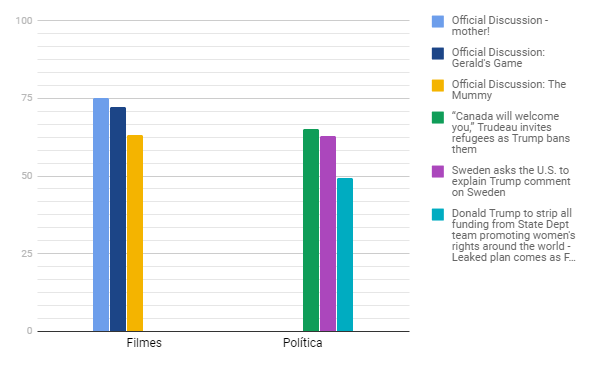
\includegraphics[height=300px]{imagens/grafico1.png}
\caption{Assertividade da ferramenta desenvolvida.}
\label{fig:ass}
\end{figure}

Através dos resultados
apresentados, pode-se verificar que a ferramenta apresentou maior assertividade
ao análisar comentários de filmes aonde o resultado se mostrou similar ao
apresentado por Pålsson e Szerszen
\cite{SentimentinSocialMedia}. 

Em relação aos tópicos relacionados a política, a ferramenta apresentou uma
baixa assertividade, chegando a apresentar assertividade similar a assertividade
obtida por classificando comentários de forma aleatória, o que naturalmente
iria classificar os comentários com 50\% de acerto eventualmente.

\newpage

Destaca-se que os tópicos de discussão de filmes encorajam o leitor a avaliar o
filme que está sendo discutido apresentando uma enquete em seu corpo, enquanto
os comentários sobre política apresentam no conteúdo de seu tópico somente um
\textit{link} direto para a notícia original. 

Como o \ac{VADER} faz uso de um
dicionário para a avaliação dos sentimentos, e nos tópicos relacionados com
política não é pedido que o autor do comentário expresse sua opinião sobre o
que estamos querendo avaliar, o \ac{VADER} acaba atribuindo sentimentos não
existentes ou com sua polaridade errada em determinadas frases, como por
exemplo: 

\textit{``\ldots What if he is just like trump and trump's useless
father\ldots``}. 

Neste caso, o dicionário irá avaliar de forma positiva o
comentário pois a palavra \textit{``like''}, quando utilizada com o significado
de ``gostar'' apresenta um sentimento positivo, porém, a palavra
\textit{``like''} neste caso está sendo utilizada como comparação, fazendo com
que a ferramenta apresente o sentimento errado.

% \chapter{Conclusão Final}
\label{cap:conclusao}
Através deste trabalho, observou-se que os métodos mais utilizados para análise
de sentimentos são o Método de Naive Bayes (estatístico) e o Método de \ac{VADER} (simbólico). Dentre
estes, optou-se pela utilização do método de \ac{VADER}, uma vez que de acordo
com a literatura, esse apresenta um desempenho superior ao método de Naive
Bayes, na análise de sentimentos nas avaliações de
produtos da Amazon, editoriais do New York Times e mais importante, na análise
de \textit{Tweets} da rede social Twitter \cite{SentimentinSocialMedia}.

A partir dos resultados obtidos verifica-se que o método de \ac{VADER} sozinho
apresenta resultados insatisfatórios. Desta forma, foi
utilizado o método de Propagação Dupla e também a escolha de palavras alvo para
a análise. 

Foram analisados 6 tópicos divididos em duas categorias,
comentários políticos e comentários de filmes. Estes tópicos foram analisados em
sua assertividade e assertividade por quantidade de caracteres. Os resultados
desta análise nos demonstrou que os comentários sobre filmes, apresentaram maior
assertividade que comentários políticos. Isso se deve ao fato de que nos tópicos relacionados com filmes, é pedido a opinião
ou avaliação dos usuários sobre aquele filme, aumentando a utilização de
expressões simples como \textit{``\ldots este filme foi ruim\ldots''}. Também, a
partir da análise de assertividade por quantidade de caracter, foi possível
demonstrar que o \ac{VADER} tende a perder assertividade quanto maior a
quantidade de caracteres em um comentário. 

De fato, quanto maior o número de
caracteres, menor a assertividade do método. Essas tendências já haviam sido
observadas nos trabalhos de Hutto e Gilbert \cite{conf/icwsm/HuttoG14}.


\section{Trabalhos Futuros}

Como sugestão de trabalhos futuros, a análise de comentários do Reddit através do
\textit{``Naive Bayes''} para que seja possível elencarmos pontos positivos e
negativos deste método em relação ao método de \ac{VADER} na sua utilização
no Reddit.

Sugere-se ainda, a incorporação do
histórico do usuário na análise de sentimentos. Ou seja, para definirmos se um
usuário está sendo irônico, por exemplo, seria interessante verificar se este
sempre elogiou determinado produto, e somente neste determinado comentário ele está criticando este.

% \include{capitulos/capitulo7}

\bibliography{tcc}
\bibliographystyle{abnt}

\end{document}